\documentclass[times]{itmo-student-thesis}

%% Опции пакета:
%% - specification - если есть, генерируется задание, иначе не генерируется
%% - annotation - если есть, генерируется аннотация, иначе не генерируется
%% - times - делает все шрифтом Times New Roman, собирается с помощью xelatex
%% - languages={...} - устанавливает перечень используемых языков. По умолчанию это {english,russian}.
%%                     Последний из языков определяет текст основного документа.

%% Делает запятую в формулах более интеллектуальной, например:
%% $1,5x$ будет читаться как полтора икса, а не один запятая пять иксов.
%% Однако если написать $1, 5x$, то все будет как прежде.
\usepackage{icomma}


%% Один из пакетов, позволяющий делать таблицы на всю ширину текста.
\usepackage{tabularx}

%% Позволяет обединять строки таблицы
\usepackage{multirow}

%% Указывает число последних букв слова, которое можно перенести на новую строку 
\righthyphenmin=2

%% Делает кавычки в листингах прямыми.
\usepackage{fontspec}
\lstset{basicstyle=\addfontfeature{Mapping=no-mapping-ligtex}}

%% Добавляет абзацные отсупы для параграфов в списках кроме первого параграфа
\usepackage{enumitem}
\setlist{listparindent=\parindent, nosep}

\lstset{
    columns=fullflexible,
    basicstyle=\ttfamily\small,
    gobble=2,
    tabsize=2,
    keywordstyle=,
}

%% Указываем файл с библиографией.
\addbibresource{bachelor-thesis.bib}

\begin{document}
\studygroup{M34351}
\title{Разработка библиотеки комбинаторных парсеров высшего порядка нечувствительных к левой рекурсии}
\author{Ступников Александр Сергеевич}{Ступников А.С.}
\supervisor{Забашта Алексей Сергеевич}{Забашта А.С.}{к.т.н.}{доцент Университета ИТМО}
\publishyear{2024}
% %% Дата выдачи задания. Можно не указывать, тогда надо будет заполнить от руки.
% \startdate{01}{сентября}{2024}
% %% Срок сдачи студентом работы. Можно не указывать, тогда надо будет заполнить от руки.
% \finishdate{31}{мая}{2024}
% %% Дата защиты. Можно не указывать, тогда надо будет заполнить от руки.
% \defencedate{15}{июня}{2024}

\addconsultant{Булычев Д.Ю.}{канд. физ.-мат. наук, доцент}

\secretary{Штумпф С.А.}

%% Задание TODO
%% Аннотация TODO

%% Эта команда генерирует титульный лист и аннотацию.
\maketitle{Бакалавр}

%% Список определений
\startdefinitionspage

\begin{enumerate}
    \item \makedefinition[язык]{Формальный язык}{множество конечных слов (строк, цепочек) над конечным алфавитом}

    \item \textbf{Формальная грамматика}~(англ. \textit{formal grammar})~--- способ описания формального языка, 
        представляющий собой четверку $\Gamma =\langle \Sigma, N, S \in N, P \subset ((\Sigma \cup N)^* N (\Sigma \cup N)^*) \times (\Sigma\cup N)^{*}\rangle$, где:
        \begin{itemize}
            \item \makedefinition{$\Sigma$}{алфавит, элементы которого называют \textbf{терминалами} (англ. \textit{terminals})}
            \item \makedefinition{$N$}{множество, элементы которого называют \textbf{нетерминалами} (англ. \textit{nonterminals})}
            \item \makedefinition{$S$}{начальный символ грамматики (англ. \textit{start symbol})}
            \item \makedefinition{$P$}{набор правил вывода (англ. \textit{production rules} или \textit{productions}) $\alpha\rightarrow \beta$}
        \end{itemize}

    \item \makedefinition[КСГ, англ. \textit{сontext-free grammar}]{Контекстно-свободная грамматика}{грамматика, у которой в 
        левых частях всех правил стоят только одиночные нетерминалы}

    \item \makedefinition[КС язык, англ. \textit{context-free language}]{Контекстно-свободный язык}{язык, задаваемый контекстно-свободной грамматикой}

    \item \makedefinition[разбор, парсинг, англ. \textit{parsing}]{Синтаксический анализ}{процесс сопоставления линейной последовательности 
        лексем (слов, токенов) формального языка с его формальной грамматикой}

    \item \makedefinition[парсер, англ. \textit{parser}]{Синтаксический анализатор}{программа, производящая ситанксический анализ}

    \item \makedefinition[англ. \textit{recogniser}]{Распознаватель}{программа, определяющая, принадлежит ли строка формальному языку}

    \item \makedefinition{Семантика языка}{это значение, которое определяется синтаксической стурктрой распознаной строки}
        
    \item \makedefinition[ввод]{Входной поток}{линейная последовательность токенов, которая передаётся парсеру для разбора}
    
    \item \makedefinition{LL(k) грамматика}{грамматика, при разборе которой на основании $k$ токенов входного потока 
        можно однозначно определить правило вывода, которое необходимо применить}

    \item \makedefinition[возврат, англ. \textit{backtracking}]{Поиск с возвратом}{техника, при которой парсер возвращает поток ввода в
        исходное состояние после попытки разбора каждого правила при разборе нетерминала}

    \item \makedefinition[LMF]{Longest match first}{принцип проектирования парсера, при котором правило,
        при разборе которого способно поглотиться наибольшее число символов входного потока, должно быть опробовано первым при разборе нетерминала языка}

    \item \makedefinition[англ. \textit{lookahead}]{Предпросмотр}{число символов входного потока, которое парсер учитывает при выборе правила в 
        рамках разбора нетерминала}

    \item \makedefinition[англ. \textit{domain-specific language}, \textit{DSL}]{Предметно-ориентированный язык}{формальный язык, специализированный для конкретной 
        области применения}

    \item \makedefinition[англ. \textit{continuation}]{Продолжение}{абстрактное представление состояния 
        программы в определённый момент, которое может быть сохранено и использовано для перехода в это состояние; 
        в качестве продолжений можно использовать функции}

    \item \makedefinition[англ. \textit{continuation passing style}, \textit{CPS}]{Стиль передачи продолжения}{это стиль 
        программирования, в котором функции вместо возвращения значений передают контроль продолжениям, которые определяют,
        что случится далее}

\end{enumerate}

%% Оглавление
\tableofcontents

%% Макрос для введения. Совместим со старым стилевиком. 
\startprefacepage
\textbf{Актуальность работы}

Различных синтаксических форм представления данных (языков программирования, DSL) становится всё больше, при этом
многие	такие языки имеют схожие структуры. В связи с этим возникает необходимость писать комбинируемые парсеры, чтобы
иметь возможность разбивать их на части и переиспользовать для разных языков. Это позволило бы ускорить время
разработки парсеров для схожих формальных языков. Кроме того, такой подход дал бы возможность разбивать крупные парсеры
для сложных формальных языков на небольшие части, удобные для долгосрочной поддержки и развития. Наиболее полно задачу
комбинации парсеров решают комбинаторные парсеры. 

Тем не менее существующие реализации комбинаторных парсеров не поддерживают произвольную композицию и параметризацию
парсеров. Это происходит в том числе из-за чувствительности большинства существующих решений к левой рекурсии. В рамках
работы решаются проблемы существующих комбинаторных парсеров. В результате работы разработан комбинаторный парсер,
нечувствительный к левой рекурсии, который поддерживает произвольную композицию и параметризацию парсеров.

\textbf{Структура работы}

\begin{enumerate}
    \item В Главе 1 представлено описание предметной области, обзор существующих решений. В конце главы сформулированы 
    цели и задачи работы.
    \item В Главе 2 представлено описание выбранного подхода, детали реализации решения.
    \item В Главе 3 представлена верификация полученных результатов, даны примеры практического применения 
    разработанного подхода.
\end{enumerate}

\chapter{ПОДХОДЫ К СИНТАКСИЧЕСКОМУ АНАЛИЗУ}

В этой главе даётся введение в область синтаксического анализа формальных языков, разбираются принятые подходы и приёмы, 
использующиеся при построении парсеров.

\section{Виды синтаксических анализаторов}\label{sec:parsing_approaches}

Для выполнения синтаксического анализа используют парсеры. По сути, парсер --- это функция из некоторого состояния в
список пар из изменённого состояния и результата, то есть функция $S \rightarrow (R \times S)^*$, где $S$
--- множество состояний, $R$ --- множество результатов. На практике состоянием обычно является поток
некоторых символов или токенов, а результатом --- дерево разбора. Есть несколько подходов к написанию парсеров. Самый
наивный --- ручное написание парсера, например, с помощью нисходящего рекурсивного спуска. Такой подход позволяет
строить производительные и тонко настраиваемые парсеры, однако, как правило, не подходит для разбора произвольных КСГ,
а также значительно увеличивает время и сложность разработки программы синтаксического анализа. Одним из более
передовых подходов является использование генераторов парсеров (таких как Bison~\cite{noauthor_bison_nodate} или
ANTLR~\cite{noauthor_antlr_nodate}), которые создают парсер на основе описания грамматики путём использования некоторого
предметно-ориентированного языка. Другим передовым подходом является использование комбинаторных парсеров, которые
представляют из себя функции, путём композиции которых пользователь неявно задаёт грамматику и семантику языка, анализ
которого будет производиться.

\section{Преимущества комбинаторных парсеров}\label{sec:parser_combinators_advantages}

Традиционно для крупных языков программирования используют генераторы парсеров, так как они за счёт выполнения
статического анализа грамматики имеют меньшее время работы. Такое время работы также достигается за счёт того, что
генераторы парсеров работают как правило только с $LL(k)$ грамматиками. Следует заметить, что такие
грамматики однозначны.

Напротив, комбинаторные парсеры зачастую способны работать с любыми контекстно-свободными грамматиками, однако при этом
имеют полиномиальное или даже экспоненциальное относительно длины ввода время работы на некоторых грамматиках и входных
данных.

Крайне важной чертой, отличающей  комбинаторные парсеры от генераторов парсеров, является интегрированность первых в
язык программирования, на котором разрабатывается иструмент, в рамках которого осуществляется синтаксический анализ.
Это  позволяет	получить  такие преимущества, как, например, проверка типов на этапе компиляции парсера. Кроме того,
такая интегрированность позволяет писать комбинаторные парсеры более абстрактно, отходя от деталей грамматики и
семантики конкретного языка программирования. Комбинаторные парсеры можно объединять произвольным образом, а части
описания этих парсеров переиспользовать.

\section{Cуществующие практические реализации комбинаторных парсеров и их проблемы}\label{sec:current_parser_combinators_problems}

Простейшая реализация комбинаторного парсера использует поиск с возвратом, чтобы имееть возможность разбирать
произвольные  КСГ. Однако использование возврата может приводить к экспоненциальному времени разбора некоторых слов
для ряда грамматик. Например, рассмотрим грамматику на рисунке~\ref{exp_grammar}.

\begin{figure}[!h]
\caption{Грамматика c экспоненциальной сложностью}\label{exp_grammar}
\[
    \begin{array}{lll}
        A & \to & xAa      \\
          &     & xAb      \\
          &     & \epsilon
    \end{array}
\]
\end{figure}

На вводах типа \lstinline[language=Haskell]{"xxxxbbbb"} (которые можно записать выражением $x^nb^n$) cложность разбора
в соответствии с грамматикой на рисунке~\ref{exp_grammar} растёт экспоненциально с ростом $n$.
Действительно, при раскрытии нетерминала $A$ парсер, использующий поиск с возвратом, сначала пытается применить первое
правило, то есть $A \to xAa$. При этом на вводах типа $x^nb^n$ при раскрытии
$A$ всегда необходимо применять второе правило. Получается, что парсер как бы перебирает в
лексикографическом порядке все строки вида $x^n(a|b)^n$ для некоторого $n$, притом строка
$x^nb^n$ будет проверена последней, а значит, парсер сделает число шагов равное числу строк вида
$x^n(a|b)^n$ минус 1, то есть для заданного $n$ парсер сделает $2^{n-1}$ шагов.

Во избежание экспоненциального времени работы некоторые практические реализации комбинаторных парсеров могут делать
возврат, только если пользователь явно укажет, что он необходим при разборе правила некоторого нетерминала (так
делает Megaprsec~\cite{noauthor_megaparsec_nodate} с помощью кобинатора try). Это позволяет достигнуть линейного времени работы,
однако использование этого подхода приводит к тому, что парсеры приходится писать с учётом LMF, что не
позволяет разбирать неоднозначные грамматики, а также приводит к невозможности описать любую КСГ. Это плохо само по
себе, однако ещё хуже то, что следствием этого является невозможность комбинировать такие парсеры, ведь при
произвольном объединении грамматик путём композиции функций-парсеров LMF может перестать
соблюдаться. Например, при объединении грамматик, состоящих из нетерминалов $A$ и
$B$ с рисунка~\ref{uncomposable_grammar}, путём задания парсера для нетерминала $C$ строку
\lstinline|"somebody"| нельзя будет полностью распознать, потому что её префикс \lstinline|"some"| будет поглощён правилом
$A \to some$, хотя грамматика из нетерминала $B$ способна поглотить весь поток ввода.

\begin{figure}[!h]
    \caption{Неправильное объединение парсеров}\label{uncomposable_grammar}
    \[
        \begin{array}{lll}
            A & \to & anybody \\
              &     & some  \\
            B & \to & somebody \\
              &     & any  \\
            C & \to & A  \\
              &     & B
        \end{array}
    \]
\end{figure}

Другим подходом, позволяющим комбинаторным парсерам с возвратом работать за время меньшее, чем экспоненциальное,
является использование мемоизации. Причина экспоненциального времени работы парсеров с возвратом (как в том числе
можно видеть из примера c рисунка~\ref{exp_grammar}) заключается в том, что одна и та же часть ввода разбирается
парсером несколько раз. Такого поведения можно избежать путём запоминания промежуточных результатов разбора парсера.
При использовании комбинаторного парсера любой нетерминал грамматики является функцией, которая принимает поток ввода и
возвращает список пар из изменённого состояния и результата. Например, парсер для нетерминала $A \to aA | \epsilon$ на
строке \lstinline{"aaa"} вернёт \lstinline{[("aaa", "")("aa", "a"), ("a", "aa"), ("", "aaa")]}. Для мемоизации парсера
$A$ необходимо завести таблицу, в которую при первом вызове парсера $A$ на
\lstinline{"aaa"} добавится запись о том, что для ввода \lstinline{"aaa"} парсер должен вернуть
\lstinline{[("aaa", "")("aa", "a"), ("a", "aa"), ("", "aaa")]}. При последующих вызовах парсера $A$ на \lstinline{"aaa"}
будет возвращаться мемоизированный результат. При условии возможности находить хеш частей входного потока и сравнивать
их за константное время эта операция выполняется за константное время. Следует заметить, что подход с мемоизацией
обладает теми же свойствами, что и хорошо известный алгоритм Эрли~\cite{earley_efficient_1970, norvig_techniques_1991} 
за исключением того факта, что мемоизированные парсеры не могут быть записаны леворекурсивно. Как следствие,
мемоизированные парсеры с возвратом способны разбрирать любую КСГ за полиномиальное время.

Тем не менее большинство мемоизированных комбинаторных парсеров с возвратом ограничены в том, как их можно
комбинировать между собой. Особенно это касается комбинаторных парсеров высшего порядка, которые на основе одних
парсеров создают другие. Одной из проблем является невозможность большинства комбинаторных парсеров завершаться при
разборе леворекурсивных грамматик.

\section{Левая рекурсия}\label{sec:left_recursion}

Левая рекурсия возникает, когда для разбора нетерминала грамматики необходимо разобрать этот же нетерминал в той же позиции. 

\begin{figure}[!h]
    \caption{Леворекурсивная грамматика}\label{leftrec_grammar}
    \[
        \begin{array}{lll}
            E & \to & E+E \\
              &     & t
        \end{array}
    \]
\end{figure}

Грамматику и семантику некоторых языков гораздо удобнее описывать с использованием левой рекурсии. Кроме того,
левая рекурсия может возникнуть при использовании комбинаторных парсеров высшего порядка. Рассмотрим пример из листинга 
\ref{lst:higher_order_left_rec}.

\begin{lstlisting}[float=!h,caption={Возникновение левой рекурсии},label={lst:higher_order_left_rec}]
    seq (x, y) = x ";" y
    stmt = seq (stmt, stmt) | VAR ":=" EXPR
\end{lstlisting}

Сам по себе парсер \lstinline{seq} нелеворекурсивен, однако при вызове его с \lstinline{stmt} в качестве первого аргумента возникает левая рекурсия.
Этот нарочито простой пример показывает, как левая рекурсия может неожиданным образом возникнуть при использовании
парсеров высшего порядка.

Таким образом, одно из главных преимуществ комбинаторных парсеров, заключающееся в их композиционности, остаётся
раскрытым не до конца в случае, когда леворекурсивные грамматики не могут быть разобраны парсером.

\section{Типы комбинаторных парсеров}\label{sec:parser_combinators_types}

Для написания комбинаторных парсеров обычно используют одну из двух абстракций: \textbf{монаду}~(англ.
\textit{monad})	или \textbf{аппликатив}~(англ. \textit{applicative}). Парсеры, которые используют эти
абстракции называют соответственно  \textbf{монадическими} и \textbf{апликативными}. Можно заметить, что тип любого
парсера (то есть $S \rightarrow (S \times R)^*$) принадлежит классу монад~\cite{hutton_monadic_1999}. Монадические парсеры
являются подмножеством апликативных, то есть с помощью монадического парсера всегда можно закодировать аппликативный.
Монадические парсеры обладают большей выразительной мощью, чем аппликативные, что позволяет с их помощью описывать не
только	    контекстно-свободные грамматики. Однако эта мощь приводит к тому, что структуру монадических парсеров
невозможно анализировать статически, что нельзя сказать об аппликативных парсерах. В листинге \ref{lst:non_context_free}
приведён пример монадического парсера,	который парсит слова из не контекстно-свободного языка, задаваемого множеством
слов $\{a^nb^nc^n \mid n \in \mathbb{N}\}$. Заметим, что структура парсера \lstinline{anbncn} формируется во время работы
программы, а не на этапе компиляции, и зависит от числа символов \lstinline{'a'}, которое присутсвует в
начале разбираемой строки.

\begin{lstlisting}[language=Haskell,float=!h,caption={Класс монад в Haskell},label={lst:monad_typeclass}]
    class Monad m where
        return :: a -> m a
        (>>=) :: m a -> (a -> m b) -> m b
\end{lstlisting}

\begin{lstlisting}[language=Haskell,caption={Класс аппликативов в Haskell},label={lst:applicative_typeclass}]
    class Applicative f where
        (<$>) :: (a -> b) -> f a -> f b
        pure :: a -> f a
        (<*>) :: f (a -> b) -> f a -> f b
\end{lstlisting}

\begin{lstlisting}[language=Haskell,caption={Монадический парсер для не КС языка},label={lst:non_context_free}]
    anbncn :: Parser String String
    anbncn = do
        a <- some (char 'a')
        b <- replicate (length a) (char 'b')
        c <- replicate (length a) (char 'c')
        return (a ++ b ++ c)
\end{lstlisting}

\section{Существующие решения}\label{sec:existing_solutions}

На текущий момент есть несколько алгоритмов синтаксического анализа, позволяющих разбирать любые леворекурсивные
контекстно-свободные грамматики с использованием комбинаторных парсеров. Рассмотрим их подробнее.

\textbf{Использование длины остатка ввода}~\cite{hudak_parser_2008}

Данный подход использует длину оставшегося ввода и специальный контекст для подсчёта числа леворекурсивных вызовов, которое
было сделано в некоторой ветви разбора. Если число леворекурсивных вызовов превышает оставшуюся длину ввода, ветвь разбора
завершается с пустым результатом. Для обеспечения полиномиального времени работы используется мемоизация. Главным недостаткамом данного 
подхода является асимптотика $O(n^4)$ для леворекурсивных грамматик. Для всех остальных грамматик асимптотика --- $O(n^3)$. Кроме
того для работы данного подхода необходимо знать длину ввода.

\textbf{Cancellation-разбор}~\cite{nederhof_new_1993}

Данный подход использует <<cancellation set>>, который хранит посещённые в текущей ветке разбора нетерминалы. C помощью <<cancellation set>>
можно отслеживать леворекурсивные вызовы нетерминалов и успешно их проводить. Недостатком разбора является экспоненциальное время работы,
а также необходимость измения грамматики, путём добавления специльных нетерминалов, которые ответствены за работу с <<cancellation set>>.

\textbf{Леворекурсивный разбор PEG}~\cite{warth_packrat_2008}

PEG --- это особый вид грамматик, которые могут быть разобраны за линейное время с использованием алгоритма
Packrat~\cite{ford_parsing_2004}. Оригинальный алгоритм не способен работать с левой рекурсией, тем не менее в него можно
добавить поддержку леворекурсивных парсеров с помощью процесса под названием <<grow the seed>>~\cite{warth_packrat_2008}, в
рамках которого леворекурсивная цепочка правил применяются к потоку ввода много раз до тех пор, пока это применение
закончивается успешно. Данная модификация сохраняет линейное время работы алгоритма. 

Такое время работы достигается в алгоритме Packrat с помощью использования мемоизации, а также за счёт особенностей
PEG, в частности того факта, что PEG локально и глобально однозначны в отличие от КСГ, которые могут быть локально
неоднозначными даже при условии глобальной однозначности.

Недостаток этого подхода заключается в том, что в PEG привычная операция альтерации между правилами нетерминалов не
является симметричной. Например, грамматика $A \leftarrow aa / a$ не эквивалетна $A \leftarrow a / aa$ (в PEG вместо
<<$|$>>{} принято писать <<$/$>>{}, а вместо <<$\to$>>{} писать <<$\leftarrow$>>):
на вводе \lstinline{"ab"} парсер для $A \leftarrow ab / b$ должен вернуть \lstinline{"ab"}, а парсер для
$A \leftarrow b / ab$ вернуть \lstinline{"a"}, потому что правило $A \leftarrow aa$ не будет применено к вводу,
так как первое завершилось успешно. Говоря иначе, парсеры для PEG не делают возврат, потому что само описание PEG делает
это невозможным. В связи с этим парсеры для PEG должны быть написаны с учётом LMF, что не позволяет их
комбинировать.

\textbf{Разбор в стиле передачи продолжений или CPS}~\cite{johnson_memoization_1995}

Джонсон предложил подход к написанию распознавателей с использованием мемоизированных продолжений. Оказывается, что
распознаватели, полученные путём   применения этого подхода нечувствительны к левой рекурсии, а также имеют время
работы $O(n^3)$. К сожалению, в оригинальный работе приводится способ строить только распознаватели, но не
парсеры. Следствием этого является использование множеств для хранения результатов разбора в оригинальной работе, что
приводит к необходимости уметь сравнивать такие результаты, а также искать их хеш за константу. Это не проблема для
распознавателей, где результатом является длина разобранного префикса ввода, однако для парсеров такое требование
неприемлемо, ведь при работе с ними пользователь сам определяет тип результата, для которого не всегда возможно
написать константную по времени реализацию сравнения и поиска хеша. Кроме того, при наивном расширении алгоритма на
парсеры время его работы становится неограниченно полиномиальным, где степень полинома зависит от размера грамматики.
Одно из решений этих двух проблем предложено в библиотеке комбинаторных парсеров Meerkat~\cite{izmaylova_practical_2016}.
Предложенное решение опирается на построение SPPF в рамках разбора. Такой подход не позволяет задавать пользователю
произвольную семантику для разбора. Тем не менее для однозначных грамматик существует способ расширить подход,
использованный в оригинальный работе Джонсона, на парсеры, в том числе на монадические комбинаторные парсеры, сохранив
возможность задания произвольной семантики разбора.

\section{Цель и задачи работы}\label{sec:goal_and_objectives}

После введения в предметную область можно поставить цель и определить задачи ВКР.

\textbf{Цель работы}

Добиться возможности произвольной композиции и параметризации парсеров.

\textbf{Задачи работы}

\begin{enumerate}
  \item Изучение литературы по теме.
  \item Создание библиотеки комбинаторных парсеров, обладающих следующими свойствами:
    \begin{enumerate}
        \item Распознавание любой однозначной контекстно-свободной грамматики.
        \item Нечувствительность к LMF.
        \item Нечувствительность к левой рекурсии.
        \item Полиномиальное время работы.
        \item Возможность задания семантики разбора.
    \end{enumerate}
  \item Оценка работы написанной библиотеки.
\end{enumerate}

\chapterconclusion

В этой главе были описаны основные подходы к созданию инструментов синтаксического анализа. Были разобраны тонкости
реализации комбинаторных парсеров, рассмотрены существующие решения. Кроме того, были поставлены цель и задачи ВКР.

\chapter{РАЗБОР В СТИЛЕ ПЕРЕДАЧИ ПРОДОЛЖЕНИЯ}

Для достижения цели, поставленной в работе, было принято решение взять за основу CPS распознаватели и усовершенствовать их.
В этой главе сначала будет рассмотрено, что такое стиль передачи продолжения в целом, далее будет описана монада продолжения,
после этого её мемоизированная версия. Наконец, будет показано, как создать парсер с помощью мемоизированной монады продолжения.

\section{Стиль передачи продолжения (CPS)}\label{sec:cps}

Для написания реализованной в рамках ВКР библиотеки был выбран язык программирования Haskell. Haskell является чистым нестрогим функциональным языком. 
Разберёмся, как устроен стиль передачи продолжения в подобном языке. Рассмотрим пример кода из листинга 
\ref{lst:pythagoras} для рассчёта квадрата гипотенузы треугольника~\cite{noauthor_haskellcontinuation_nodate} по теореме Пифагора.

\begin{lstlisting}[language=Haskell,float=!h,caption={Теорема Пифагора},label={lst:pythagoras}]
    add :: Int -> Int -> Int
    add x y = x + y

    square :: Int -> Int
    square x = x * x

    pythagoras :: Int -> Int -> Int
    pythagoras x y = add (square x) (square y)
\end{lstlisting}

Чтобы записать тот же код в CPS необходимо, чтобы функции \lstinline[language=Haskell]{add},
\lstinline[language=Haskell]{square} и \lstinline[language=Haskell]{pythagoras} вместо \lstinline[language=Haskell]{Int}
возвращали функцию, которая принимает продолжение и возвращает результат, эту функцию будем называть \textit{отложенным вычислением}. Тип такой функции \lstinline[language=Haskell]{(Int -> r) -> r}, 
то есть само продолжение имеет тип \lstinline[language=Haskell]{Int -> r}. Код, переписанный в стиле передачи продолжения, 
представлен на листинге \ref{lst:pythagoras_cps}. Можно сказать, что теперь все функции принимают дополнительный аргумент 
с типом \lstinline[language=Haskell]{Int -> r}, который является продолжением.

\begin{lstlisting}[language=Haskell,float=!h,caption={Теорема Пифагора в CPS},label={lst:pythagoras_cps}]
    add_cps :: Int -> Int -> ((Int -> r) -> r)
    add_cps x y = \k -> k (add x y)
    
    square_cps :: Int -> ((Int -> r) -> r)
    square_cps x = \k -> k (square x)
    
    pythagoras_cps :: Int -> Int -> ((Int -> r) -> r)
    pythagoras_cps x y = \k ->
        square_cps x $ \x_squared ->
        square_cps y $ \y_squared ->
        add_cps x_squared y_squared $ k
\end{lstlisting}

Теперь, чтобы получить результат вычислений, например, для треугольника с катетами 3 и 4, можно вызвать \lstinline[language=Haskell]{pythagoras_cps 3 4 id}.

\subsection{Монада Cont}\label{sec:cps_monad}

Пусть необходимо последовательно соединить два
отложенных вычисления \lstinline[language=Haskell]{(a -> r) -> r} и \lstinline[language=Haskell]{(b -> r) -> r}, 
притом второе вычисление хочется составлять на основе первого. Функция для этого представлена на листинге \ref{lst:cps_bind}.

\begin{lstlisting}[language=Haskell,float=!h,caption={Соединение отложенных вычислений},label={lst:cps_bind}]
    chainCPS :: ((a -> r) -> r) -> 
        (a -> ((b -> r) -> r)) -> 
        ((b -> r) -> r)
    chainCPS s f = \k -> s $ \x -> f x $ k
\end{lstlisting}

Заметим, что если заменить \lstinline[language=Haskell]{(a -> r) -> r} на \lstinline[language=Haskell]{m a}, а 
\lstinline[language=Haskell]{(b -> r) -> r} на \lstinline[language=Haskell]{m b}, то функция \lstinline[language=Haskell]{chainCPS}
по сути будет являться монадическим \lstinline[language=Haskell]{bind}.

Разовьём эту идею, добавив новый тип c листинга \ref{lst:cont_type}.

\begin{lstlisting}[language=Haskell,float=!h,caption={Тип Cont},label={lst:cont_type}]
    newtype Cont r a = Cont { 
        runCont :: (a -> r) -> r 
        }
\end{lstlisting}

По сути тип \lstinline[language=Haskell]{Cont} --- это обёртка над функцией \lstinline[language=Haskell]{(a -> r) -> r}.
Этот тип является монадой, что показано на листинге \ref{lst:cont_monad}.

\begin{lstlisting}[language=Haskell,float=!h,caption={Включение типа Cont в класс Monad},label={lst:cont_monad}]
    instance Monad (Cont r) where
        return x = Cont ($ x)
        s >>= f  = Cont $ \c -> runCont s $ 
                    \x -> runCont (f x) c
\end{lstlisting}

\subsection{Монада продолжения полиморфная по результату}\label{sec:poly_cont_monad}

Недостаток монады Cont с листинга \ref{lst:cont_type} заключается в том, что тип результата (то есть
\lstinline{r}) должен оставаться  неизменным внутри монады. Это означает, что при использовании функции \lstinline{bind} нельзя изменить 
тип результа монады, что не позволяет, например, при описании парсеров соединять через \lstinline{bind} парсеры,
возвращающие разные по типу результаты. Чтобы это исправить нужно, чтобы тип результата определялся не типом
\lstinline{Cont}, а типом продолжения \lstinline{a -> r}. Для этого воспользуемся Haskell.
Обновленная версия типа \lstinline{Cont}, которая полиморфна по результату, а также включение \lstinline{Cont} в класс монад
для неё  представлен  на листинге \ref{lst:poly_cont_monad}. Можно заметить, что определение включения \lstinline{Cont} 
в класс монад не изменилось.

\begin{lstlisting}[language=Haskell,float=!h,caption={Монада продолжения полиморфная по результату},label={lst:poly_cont_monad}]
    newtype Cont a = Cont
        { runCont :: forall r. (a -> r) -> r
        }

    instance Monad (Cont r) where
        return x = Cont ($ x)
        s >>= f  = Cont $ \c -> runCont s $ 
                    \x -> runCont (f x) c
\end{lstlisting}

\subsection{Монада продолжения с состоянием}\label{sec:stateful_cont}

Для написания мемоизированного парсера в CPS необходимо, чтобы отложенные вычисления использовали таблицу мемоизации. 
Такая таблица мемоизации является по сути изменяемым состоянием. Для его реализации можно воспользоваться монадой состояния.
Тогда тип \lstinline{Cont} необходимо изменить. Изменённый тип представлен на листинге \ref{lst:stateful_cont_type}.

\begin{lstlisting}[language=Haskell,float=!h,caption={Тип Cont с состоянием},label={lst:stateful_cont_type}]
    newtype Cont a = Cont { 
        runCont :: forall r. (a -> State MemoTable r) 
            -> State MemoTable r 
        }
\end{lstlisting}

Теперь продолжения имеют тип \lstinline{a -> State MemoTable r} и могут использовать таблицу мемоизации для вычисления результата.
Класс Monad для нового типа продолжений определяется так же, как на листинге \ref{lst:poly_cont_monad}.

\subsection{Недетерминированная монада продолжения}\label{sec:contt_transformer}

В результате работы парсера может получится несколько результатов или вовсе ни одного, что свидетельствует о том, что 
разбираемая строка не принадлежит языку. Поэтому отложенные вычисления в монаде \lstinline{Cont} должны возвращать не 
единственный результат (как это следовало из типа \lstinline{Cont} до сих пор), а коллекцию результатов. В качестве коллекции используем обычный список.
Снова изменим тип \lstinline{Cont}, заменив тип результата \lstinline{r} на \lstinline{[r]}. Изменённый тип представлен на листинге \ref{lst:nondeterministic_cont_type}.
Важно заметить, что изменённый тип принадлжит классу Alternative.

\begin{lstlisting}[language=Haskell,float=!h,caption={Недетерминированная монада продолжения с состоянием},label={lst:nondeterministic_cont_type}]
    newtype Cont a = Cont { 
        runCont :: forall r. (a -> State MemoTable [r]) 
            -> State MemoTable [r] 
        }

    instance Alternative Cont where
        empty :: Cont a
        empty = Cont (\_ -> return empty)
        (<|>) :: Cont a -> Cont a -> Cont a
        (<|>) l r =
        Cont
            ( \k -> do
                r1 <- runCont l k
                r2 <- runCont r k
                return $ r1 <|> r2
            )
\end{lstlisting}

\section{CPS-парсеры}\label{sec:cps_parser}

Теперь с использованием разработанной в разделе \ref{sec:contt_transformer} \lstinline{Cont} монады несложно написать парсер в стиле 
передачи продолжения. Как уже было замечено ранее парсер --- это функция типа \lstinline{s -> [(r, s)]}, где \lstinline{s} --- это
тип потока ввода, а \lstinline{r} --- тип результата разбора. Если возвращаемый список пустой, то разбираемая строка не принадлежит
языку, если возвращаемый список содержит более одного элемента, то строка может быть разобрана несколькими способами.
На самом деле парсер не обязан возвращать список. Например, вместо списка парсер может возвращать Maybe (листинг \ref{lst:maybe}).
В этом случае его тип --- \lstinline{s -> Maybe (r, s)}. Парсер с таким типом может возвращать \lstinline{Nothing}, если разбор 
закончился неудачно, или \lstinline{Just (r, s)}, если разбор завершился успехом. Заметим, что такой парсер не может вернуть 
несколько результатов разбора. Подробнее с этим можно ознакомиться в рамках работы~\cite{hutton_monadic_1999}.

\begin{lstlisting}[language=Haskell,float=!h,caption={Тип Maybe в Haskell},label={lst:maybe}]
  data Maybe a = Just a | Nothing
\end{lstlisting}

Такая независимость парсера от контейнера для результата наводит на мысль написать обобщённый тип парсера,
параметризированный относительно типа такого контейнера: \lstinline {type ParserT m s r = s -> m (r, s)}. Полученный
тип в точности соответствует монадическому трансформеру \lstinline{StateT} из Haskell (листинг \ref{lst:stetet}). При условии, что	тип
\lstinline{m} принадлежит классу монад, тип \lstinline{StateT} также принадлежит к классу монад. 

\begin{lstlisting}[language=Haskell,float=!h,caption={StateT трансформер монад},label={lst:stetet}]
  newtype StateT s m a = StateT (s -> m (a, s))
\end{lstlisting}

Получается, что любой монадический парсер с типом ввода \lstinline{s} и типом результата \lstinline{r} можно
записать, как \lstinline{StateT s m r}, где \lstinline{m} --- это некоторый тип, принадлежащий классу монад. Как можно 
было заметить на примере со списком и \lstinline{Maybe}, тип \lstinline{m} определяет свойства парсера. 
Тип \lstinline{Cont} из раздела \ref{sec:contt_transformer} является монадой, а значит, значения с типом
\lstinline{StateT s Cont r} являются монадическими парсерами. Такие монадические парсеры будем называть парсеры
в CPS. Введём для них тип с именем \lstinline{Parser}, как на листинге \ref{lst:cps_parser}. Тип результата
\lstinline{r} опущен, чтобы кайнд полученного типа был \lstinline{* -> *} и \lstinline{Parser} принадлежал к
классу монад (в Haskell частично параметризованные типы не поддерживаются).

\begin{lstlisting}[language=Haskell,float=!h,caption={Парсер в CPS},label={lst:cps_parser}]
  type Parser s = StateT s Cont
\end{lstlisting}

\subsection{Алгоритм разбора с левой рекурсией}\label{sec:memoized_cps_parser}

Проблема с комбинаторными парсерами, написанными леворекурсивно, заключается в том, что такие парсеры вызывают сами
себя, при этом не меняя состояние разбора. В связи с этим код производит леворекурсивные вызовы, пока не переполнится стек 
вызовов и программа не завершится с ошибкой.

Чтобы избежать подобного исхода, можно сделать следующее в случае, когда разбор нетерминала приводит к леворекурсивному вызову:
\begin{enumerate}
    \item Не производить леворекурсивный вызов, при этом сохранив цепочку парсеров, которая должена была быть вызвана после него.
    \item Когда у нетерминала, разбор которого привёл к леворекурсивному вызову, появляется новый результат, вызвать сохранённые цепочки парсеров
          на этом результате.
\end{enumerate}
Заметим, что если при вызове сохранённой цепочки парсеров у нетерминала, разбор которого привёл к леворекурсивному вызову,
появляется новый результат, то надо снова вызвать сохранённые цепочки парсеров на этом результате. 

\begin{figure}[!h]
  \caption{Леворекурсивная грамматика}\label{leftrec_grammar_cps}
  \[
      \begin{array}{lll}
          A & \to & Aa \\
            &     & b
      \end{array}
  \]
\end{figure}

Чтобы лучше понять описанный алгоритм, рассмотрим пример. Взглянем на грамматику на рисунке \ref{leftrec_grammar_cps}.
Парсер для этой грамматики принимает строки вида $ba^*$. Если придерживаться описанного алгоритма, то
парсер для нетерминала $A$ на строке \lstinline{"baa"} сначала попытается вызвать самого себя.
При этом алгоритм должен определить, что произошёл леворекурсивный вызов и не вызывать парсер, а вместо этого сохранить то, что
должно разпознаться после вызова \lstinline{A}, то есть парсер для терминала $a$. Потом
парсер для нетерминала \lstinline{A} попытается вызвать парсер для терминала \lstinline{b}, этот парсер вернёт результат
\lstinline{("b", "aa")}. Получается, что у нетерминала $A$ появился новый результат, значит, на этом
результате нужно солгасно алгоритму вызвать сохранённый парсер, то есть парсер для терминала $a$,
который вернёт результат \lstinline{("ba", "a")}. У нетерминала $A$ снова появился новый результат,
значит, на нём снова нужно вызвать парсер для $a$, который вернёт результат \lstinline{("baa", "")}.
Таким образом парсер, следуя описанному ранее алгоритму, смог разобрать всю входную строку, несмотря на левую рекурсию.

\subsection{Алгоритм работы мемоизированных CPS-парсеров}\label{sec:cps_algorithm}

Работа, проделанная в предыдущих разделах, была необходима для того, чтобы мемоизировать парсеры так, чтобы они поддерживали
левую рекурсию. 

По сути алгоритм, который был описан в разделе \ref{sec:memoized_cps_parser} и есть алгоритм работы мемоизированных CPS-парсеров. 
При этом цепочка парсеров, которая должна быть вызвана после леворекурсивного вызова, есть продолжение парсера, 
который к этому вызову привёл. В связи с этим алгоритм можно описать следующим образом, теперь уже без упора на левую рекурсию.
\begin{enumerate}
    \item Для каждого парсера нетерминала храним список его результатов и список его продолжений.
    \item При появлении у парсера нового продолжения вызываем его на всех результатах.
    \item При появлении у парсера нового результата вызываем на нём все продолжения.
\end{enumerate}

Важно заметить, что подобный алгоритм не только позволяет записывать парсеры леворекурсивно, но и гарантирует
полиномиальное время работы парсера. Чтобы убедиться в этом, обратимся к источникам. В статье, где впервые был предложен подобный алгоритм для CPS
распознавателей~\cite{johnson_memoization_1995}, утверждается, что он работает  за полиномиальное время. Алгоритм для парсеров
производит те же самые шаги, что и алгоритм для распознавателей, следовательно,  должен также работать за полиномиальное
время. Кроме того, в статье, где была разработана другая библиотека CPS-парсеров под названием Meerkat~\cite{izmaylova_practical_2016},  доказывается,
что CPS-парсеры работают за полином, притом для не сильно неоднозначных грамматик это время ограничено
$O(n^3)$. Наконец, нужно сказать, что представленный алгоритм является частным случаем мемоизированных
парсеров. В статье~\cite{norvig_techniques_1991} доказывается, что свойства мемоизированных парсеров аналогичны свойствам
парсеров Эрли.

\subsection{Реализация алгоритма CPS-парсеров}

На листингах \ref{lst:cps_types} и \ref{lst:cps_memoization} представлен основной код, необходимый для работы мемоизированных CPS-парсеров. Напомним,
что тип \lstinline{Cont} принадлежит классу монад, как это было показано ранее.

Два типа \lstinline{MemoEntry} и \lstinline{MemoTable} с листинга \ref{lst:cps_types} используются для мемоизации.
Тип \lstinline{MemoTable} --- это тип таблицы мемоизации, из этой таблицы по ключу, который уникально идентифицирует
парсер, а также вводу можно получить значение типа \lstinline{MemoEntry}. \lstinline{MemoEntry} хранит результаты
применения парсера с ключом к некоторому вводу, а также продолжения этого парсера на этом вводе, то есть по сути
парсеры, которые могут быть вызваны после парсера,
\lstinline{MemoEntry} которого рассматривается. \lstinline{MemoTable} используется в качестве состояния для \lstinline{Cont}. Для
удобства также введён тип \lstinline{ContState}, который является типом результата мемоизированного продолжения.
Введённый на листинге \ref{lst:cps_parser} тип \lstinline{Parser} переименован в \lstinline{BaseParser}, далее станет
понятно для чего.

Можно заметить, что в коде используется тип \lstinline{Dynamic} (на листинге \ref{lst:cps_types}), а также функции
\lstinline{fromDynUnsafe}, \lstinline{toDyn} и \lstinline{toDynContinuation} (на листинге \ref{lst:cps_memoization}).
Они необходимы, потому что таблица мемоизации должна хранить значения разных типов, и используются для приведения
типов, что на Haskell можно сделать с использованием \lstinline{Dynamic}~\cite{noauthor_datadynamic_nodate}.

\begin{lstlisting}[language=Haskell,float=!h,caption={Типы для CPS-парсера},label={lst:cps_types}]
  data MemoEntry k s a r = MemoEntry
  { results :: [(a, s)],
    continuations :: [(a, s) -> ContState k s [r]]
  }

  type MemoTable k s =
    Map.HashMap
      k
      (Map.HashMap s (MemoEntry k s Dynamic Dynamic))

  type ContState k s = State (MemoTable k s)

  newtype Cont k s a = Cont
    { runCont ::
        forall r.
        (Typeable r) =>
        (a -> ContState k s [r]) ->
        ContState k s [r]
    }

  type BaseParser k s = StateT s (Cont k s)
\end{lstlisting}

\begin{lstlisting}[language=Haskell,float=!h,caption={Мемоизация для CPS-парсера},label={lst:cps_memoization}]
  baseMemo ::
    (Typeable a, Hashable k, Hashable s, Eq k, Eq s) =>
    k -> BaseParser k s a -> BaseParser k s a
  baseMemo key parser = StateT $ \state ->
    Cont $ \continuation ->
      do
        modify (Map.insertWith (\_ old -> old) key Map.empty)
        entry <- gets $
          \table -> Map.lookup state $ table Map.! key
        case entry of
          Nothing -> do
            modify $
              addNewEntry state $
                MemoEntry [] [toDynContinuation continuation]
            runCont
              (runStateT parser state)
              ( \result -> do
                  modify (addResult state result)
                  conts <- gets $ \table ->
                    continuations $ (table Map.! key) Map.! state
                  join <$> mapM
                    ( \cont ->
                        fmap fromDynUnsafe <$> cont (first toDyn result)
                    )
                    conts
              )
          Just foundEntry -> do
            modify (addContinuation state continuation)
            join <$> mapM
              (continuation . first fromDynUnsafe)
              (results foundEntry)
\end{lstlisting}

На листинге \ref{lst:cps_memoization} определена функция \lstinline{baseMemo}, которая делает из обычного парсера
мемоизированный. Она принимает уникальный ключ и парсер  для мемоизации. Когда мемоизированный парсер вызывается
впервые, в таблице мемоизации по ключу для этого парсера создаётся пустой словарь, это просходит в строке
\lstinline{modify (Map.insertWith (\_ old -> old) key Map.empty)}. Далее проверяется, есть ли в этом словаре запись для 
входа, на котором был вызван парсер.

Если такой записи нет, то она создаётся путём вызова функции \lstinline{addNewEntry}, в запись сразу же помещается продолжение, с
которым был вызван мемоизированный парсер. Далее вызывается сам парсер с особым продолжением. Это продолжение
по завершении парсера с некоторым результатом сохраняет этот результат в \lstinline{MemoEntry}, а также вызывает все
сохранённые продолжения парсера на полученном результате и возвращает их результаты, соединённые в единый список.

Если запись в таблице мемоизации по ключу парсера и вводу есть, то в неё добавляется переданное в парсер продолжение, это происходит
путём вызова функции \lstinline{addContinuation}. Далее это продолжение вызывается на всех сохранённых результатах парсера.

Можно заметить, что сам мемоизированный парсер для заданного ввода вызывается единожды, далее используются его
сохранённые результаты, этим и объясняется полиномиальное время работы алгоритма.

\subsection{Пример использования CPS-парсера}\label{sec:cps_parser_example}

Покажем, как использовать написанный парсер. Сделаем это на примере грамматики с рисунка \ref{leftrec_grammar_cps}.
Для этого сначала введём примитивный парсер, который разбирает переданную в него строку. Его можно найти на листинге
\ref{lst:string_parser}. Функция stripPrefix импортирована из модуля Data.List стандартной библиотеки Haskell. Для
наглядности в качестве потока ввода в парсере используется String,  это далеко не самое удачное решение с точки зрения
производительности, библиотека позволяет использовать и другие, более эффективные потоки ввода.

\begin{lstlisting}[language=Haskell,float=!h,caption={Парсер для строки},label={lst:string_parser}]
  string :: String -> BaseParser k String String
  string s =
    StateT
      ( \state ->
          case stripPrefix s state of
            Just s' -> return (s, s')
            Nothing -> empty
      )
\end{lstlisting}

Теперь можно написать парсер для грамматики с рисунка \ref{leftrec_grammar_cps}. Он представлен на листинге
\ref{lst:baa_parser}.	В качестве ключа для парсера используется целое число $1$. Ввиду того, что
парсер единственный, ключ может быть любым. Главное, чтобы тип ключа поддерживал проверку на равенство, а также поиска
хеша за $O(1)$. Для написания парсера \lstinline{baa} использован тот факт, что любая монада
является также функтором и апликативом. Это значит, что для парсеров определены операторы
\lstinline{<$>} и \lstinline{<*>}.

\begin{lstlisting}[language=Haskell,float=!h,caption={Парсер для строк $ba^*$},label={lst:baa_parser}]
  baa :: BaseParser Int String String
  baa =
    baseMemo 1 $
      (++) <$> baa <*> chunk "a"
        <|> chunk "b"
\end{lstlisting}

\section{Генерация ключей мемоизации}\label{sec:memoization_keys}

\subsection{Парсеры первого порядка}

Расставлять ключи мемоизации вручную неудобно. Более того, при таком подходе сложно обеспечить уникальность ключей. Поэтому
необходимо предоставить средства для автоматической генерации ключей мемоизации. Для этого добавим новый тип \lstinline{Key} 
с листинга \ref{lst:memo_key_type}. \lstinline{Key} позволяет сравнивать значения разных типов. 

\begin{lstlisting}[language=Haskell,float=!h,caption={Тип ключей мемоизации},label={lst:memo_key_type}]
  data Key = forall a. (Typeable a, Hashable a, Eq a) => Key a

  instance Eq Key where
      (==) :: Key -> Key -> Bool
      (==) (Key a) (Key b) =
          case cast b of
              Just x -> a == x
              Nothing -> False

  instance Hashable Key where
      hashWithSalt :: Int -> Key -> Int
      hashWithSalt s (Key a) = hashWithSalt s a

  makeStableKey :: (Typeable a) => a -> Key
  makeStableKey a = Key (unsafePerformIO $ makeStableName a)
\end{lstlisting}

На том же листинге \ref{lst:memo_key_type} введена функция \lstinline{makeStableKey a}, которая генерирует ключ на основе
\lstinline{StableName}~\cite{noauthor_systemmemstablename_nodate}
своего аргумента. Для аргументов с одинаковыми адресами в памяти функция \lstinline{makeStableKey} возвращает равные ключи,
при этом функция также может вернуть равные ключи для равных аргументов, даже если у этих аргументов разные адреса в
памяти. Так происходит из-за оптимизаций компилятора, это не мешает использованию \lstinline{makeStableKey} по назначению.
Предполагается, что функция makeStableKey будет вызываться с функциями-парсерами в качестве аргумента, чтобы
сгенерировать ключ для этого парсера, как это сделано на листинге \ref{lst:makeStableKey_example}.

\begin{lstlisting}[language=Haskell,float=!h,caption={Пример использования makeStableKey},label={lst:makeStableKey_example}]
  baa :: BaseParser Key String String
  baa =
    baseMemo (makeStableKey baa) $
      (++) <$> baa <*> chunk "a"
        <|> chunk "b"
\end{lstlisting}

Теперь можно ввести функцию \lstinline{memo}, которая будет автоматически генерировать ключи. Закодируем парсер \lstinline{baa} c её
помощью, как на листинге \ref{lst:memo}.

\begin{lstlisting}[language=Haskell,float=!h,caption={Memo с автоматическим ключом},label={lst:memo}]
  memo :: 
    (Typeable s, Typeable a, Hashable s, Eq s) => 
    Parser s a -> Parser s a
  memo p = baseMemo (makeStableKey p) (parser p)

  baa :: BaseParser Key String String
  baa =
    memo $
      (++) <$> baa <*> chunk "a"
        <|> chunk "b"
\end{lstlisting}

\subsection{Парсеры высшего порядка}

Функция \lstinline{memo} отлично работает для парсеров первого порядка, однако её невозможно использовать с
парсерами высшего порядка. Для примера представим, что необходимо мемоизировать парсер
\lstinline{count p n} с листинга \ref{lst:count_parser}, который  принимает два аргумента: парсер и число раз,
которое этот парсер необходимо последовательно применить к вводу. Чтобы мемоизировать этот парсер, в качестве ключа
можно было бы использовать что-то похожее на \lstinline{Key (makeStableKey count, makeStableKey p, n)}, то есть тройку из
адреса самого парсера \lstinline{count}, адреса его аргумента \lstinline{p} и числа n. Так как все три элемента тройки поддерживают
операцию равенста и хеширования, то и тройка тоже её поддерживает, притом за $O(1)$. Мемоизированная версия \lstinline{count} называется \lstinline{mCount}
на листинге \ref{lst:count_parser}.

\begin{lstlisting}[language=Haskell,float=!h,caption={Парсер высшего порядка count},label={lst:count_parser}]
  count :: 
    BaseParser Key String String -> 
    Int -> 
    BaseParser Key String String
  count p n = join <$> replicateM n p

  mCount :: 
    BaseParser Key String String -> 
    Int -> 
    BaseParser Key String String
  mCount p n = baseMemo 
    (Key (makeStableKey mCount, makeStableKey p, n)) $ 
      join <$> replicateM n p
\end{lstlisting}

Тем не менее в таком подходе есть проблема. Предположим, что написан парсер \lstinline{joinedCount n = mCount (mCount (string "a") 3) n}.
Такой пример кажется несколько надуманным, однако суть его в том, что в \lstinline{mCount} подставляется парсер высшего порядка.
Теперь для первого аргумента внешнего \lstinline{mCount} неправильным будет вызывать \lstinline{makeStableKey (mCount (string "a") 3)}, потому что
этот вызов каждый раз будет возвращать новый ключ, для одинаковых парсеров, ведь \lstinline{mCount (string "a") 3} создаётся заново при каждом вызове
(если не вмешаются оптимизации компилятора, на которые в общем случае рассчитывать нельзя).

Чтобы избежать такой ситуации необходимо в парсере \lstinline{mCount} для мемоизации вместо \lstinline{makeStableKey p}
использовать ключ парсера \lstinline{p}. Для этого в каждом парсере необходимо хранить его ключ. Введём новый тип парсера на листинге \ref{lst:memoized_parser_type}. 

\begin{lstlisting}[language=Haskell,float=!h,caption={Тип парсера с ключом},label={lst:memoized_parser_type}]
  data Parser s a = Parser
    { key :: Maybe Key,
      parser :: BaseParser Key s a
    }
\end{lstlisting}

Очевидно, что тип \lstinline{Parser} принадлежит классу монад. При операциях \lstinline{fmap},
\lstinline{pure}, \lstinline{<*>}, \lstinline{>>=}, \lstinline{<|>} для созданного парсера
ключ равен \lstinline{Nothing}. Так сделано по двум причинам. Первая причина --- невозможность сравнивать функции по
значению, это приводит к невозможности сгенерировать ключи мемоизации для комбинаторов, которые принимают произвольные
функции, таких как \lstinline{fmap}, \lstinline{<*>} и \lstinline{>>=}. Примерно по той же причине ключ не
генерируется для  комбинатора \lstinline{pure}, в \lstinline{pure} передаётся некоторый результат парсера, на этот
результат не хочется налагать ограничения на возможность проверки на равенство и поиска хеша. Вторая причина, по
которое некоторые ключи равны \lstinline{Nothing} --- производительность. Например, для комбинатора \lstinline{<|>}
ключ нужно генерировать на основе двух его аргументов-парсеров, таким образом, ключ получается вложенным, время сравнения таких ключей потенциально 
может зависеть от размера грамматики. 

Для других парсеров в том числе \lstinline{empty} и некоторых примитивных парсеров, таких как
\lstinline{string}, ключ генерируется на основе аргументов. То есть, например, все парсеры \lstinline{string} для
одинаковых строк имеют одинаковые ключи. Введём для удобства две новые функции, ответственные за мемоизацию:
\lstinline{memo} и \lstinline{memoWithKey}. Теперь можно переопределить
\lstinline{mCount}. Функции \lstinline{memo}, \lstinline{memoWithKey} и обновлённый \lstinline{mCount} представлены на
листинге \ref{lst:mcount_fixed}. Для парсеров высшего порядка всегда необходимо указывать ключи явно.

\begin{lstlisting}[language=Haskell,float=!h,caption={Исправленный mCount},label={lst:mcount_fixed}]
  memo :: 
    (Typeable s, Typeable a, Hashable s, Eq s) => 
    Parser s a -> Parser s a
  memo p = Parser k (baseMemo k (parser p))
    where
    k = makeStableKey p

  memoWithKey :: 
    (Typeable s, Typeable t, Hashable s, Eq s) => 
    Key -> Parser s t -> Parser s t
  memoWithKey k p = Parser k (baseMemo k (parser p))

  getOrMakeKey :: (Typeable s,Typeable a)=>Parser s a -> Key
  getOrMakeKey (Parser (Just k) _) = k
  getOrMakeKey p@(Parser Nothing _) = makeStableKey p

  mCount :: 
    Parser String String -> 
    Int -> 
    Parser String String
  mCount p n = memoWithKey 
    (Key (makeStableKey mCount, getOrMakeKey p, n)) $ 
      join <$> replicateM n p
\end{lstlisting}

\chapterconclusion

В этой главе были проанализированы существующие алгоритмы, с помощью которых потенциально возможно достичь цели ВКР. 
Был выбран и доработан наиболее удачный алгоритм. Далее доработанный алгоритм был практически реализован с использованием 
языка программирования Haskell.

\chapter{СВОЙСТВА CPS-ПАРСЕРОВ}

В этой главе рассматриваются результаты, полученные в рамках второй главы. В том числе время работы полученного парсера,
возможности его практического применения, а также ограничения. 

\section{Разбор арифметических выражений}\label{sec:arith_expr}

Для оценки времени работы закодируем с использованием разработанной библиотеки парсер для языка арфметических
выражений, заданного грамматикой с листинга  \ref{fig:expr_grammar}. В качестве семантики языка используем
алгебраические типы данных с листинга \ref{lst:expr_semantics}. Сам парсер представлен на листинге \ref{lst:expr_parser}.
Заметим, что код парсера в точности соответсвует грамматике, несмотря на то, что она леворекурсивна. Это достигается за счёт
использования функции \lstinline{memo} при написании парсеров \lstinline{f}, \lstinline{term} и \lstinline{expr}.

\begin{figure}[!h]
  \caption{Грамматика арифметических выражений}\label{fig:expr_grammar}
  \[
      \begin{array}{lll}
          F & \to & number \\
            &     & (E) \\
          T & \to & T * F \\
            &     & T / F \\
          E & \to & E + T \\
            &     & E - T
      \end{array}
  \]
\end{figure}

\begin{lstlisting}[language=Haskell,float=!h,caption={Семантические значения языка арифметических выражений},label={lst:expr_semantics}]
  data Expr = ExprOp Expr String Term | ExprVal Term

  data Term = TermOp Term String F | TermVal F

  data F = FExpr Expr | FVal Int
\end{lstlisting}

\begin{lstlisting}[language=Haskell,float=!h,caption={Парсер арифметических выражений},label={lst:expr_parser}]
  f :: Parser (ParserState T.Text) F
  f =
    memo $
      FVal . either undefined fst . decimal <$> regex "[0-9]+"
        <|> FExpr <$> (single '(' *> expr <* single ')')

  term :: Parser (ParserState T.Text) Term
  term =
    memo $
      TermVal <$> f
        <|> TermOp <$> term <*> (pure <$> oneOf ['*', '/']) <*> f

  expr :: Parser (ParserState T.Text) Expr
  expr =
    memo $
      ExprOp <$> expr <*> (pure <$> oneOf ['+', '-']) <*> term
        <|> ExprVal <$> term

  exprStart :: Parser (ParserState T.Text) Expr
  exprStart = expr <* eof
\end{lstlisting}

Для сравнения парсер для языка арифметических выражений также был написан с использованием Megaparsec~\cite{noauthor_megaparsec_nodate}.
Так как  Megaparsec не поддерживает левую рекурсию, грамматика для арифметических выражений предварительно была
переписана в нелеворекурсивную форму тривиальным образом. 

Помимо этого для нелеворекурсивной грамматики был написан парсер с использованием разработанной библиотеки, который не
использует функцию \lstinline{memo}. Это возможно, так как грамматика арифметических выражений принадлежит классу
грамматик $LL(1)$, а значит, её возможно разобрать без использования поиска с возвратом. Вместе с тем
переписанная грамматика нелеворекурсивна. Всё это делает использование мемоизации необязательным.

На рисунке \ref{fig:expr_plot} представлено время работы написанных парсеров в зависимости от длины разбираемого
арифметического выражения. График <<Memo CPS>> показывает время работы мемоизированного CPS-парсера, график
<<Megaparsec>> --- время работы  парсера на Megaparsec,  график <<CPS>> --- время работы CPS-парсера без мемоизации и
возврата. По графику <<Memo CPS>> видно, что разработанная библиотека разбирает арифметические выражения, записанные 
леворекурсивно, за линейное время. Предположительно, линейное время работы будет наблюдаться на всех детерминированных грамматиках,
как в случае с алгоритмом Эрли.

Тем не менее время работы мемоизированного парсера много больше времени работы парсера,
закодированного с использованием Megaparsec. Такие различия объясняются необходимостью поиска в хеш-словаре, а также 
недетерминированностью оператора выбора (\lstinline{<|>}). Вместе с тем по графику <<CPS>> видно, что разработанная библиотека
поддерживает написание парсеров в виде, при котором скорость работы сравнима со скоростью работы парсера на Megaparsec. Это
достигается путём отказа от мемоизации и использования детерминированного оператора выбора.

\begin{figure}[!h]
  \caption{Скорость работы парсеров арифметических выражений}\label{fig:expr_plot}
  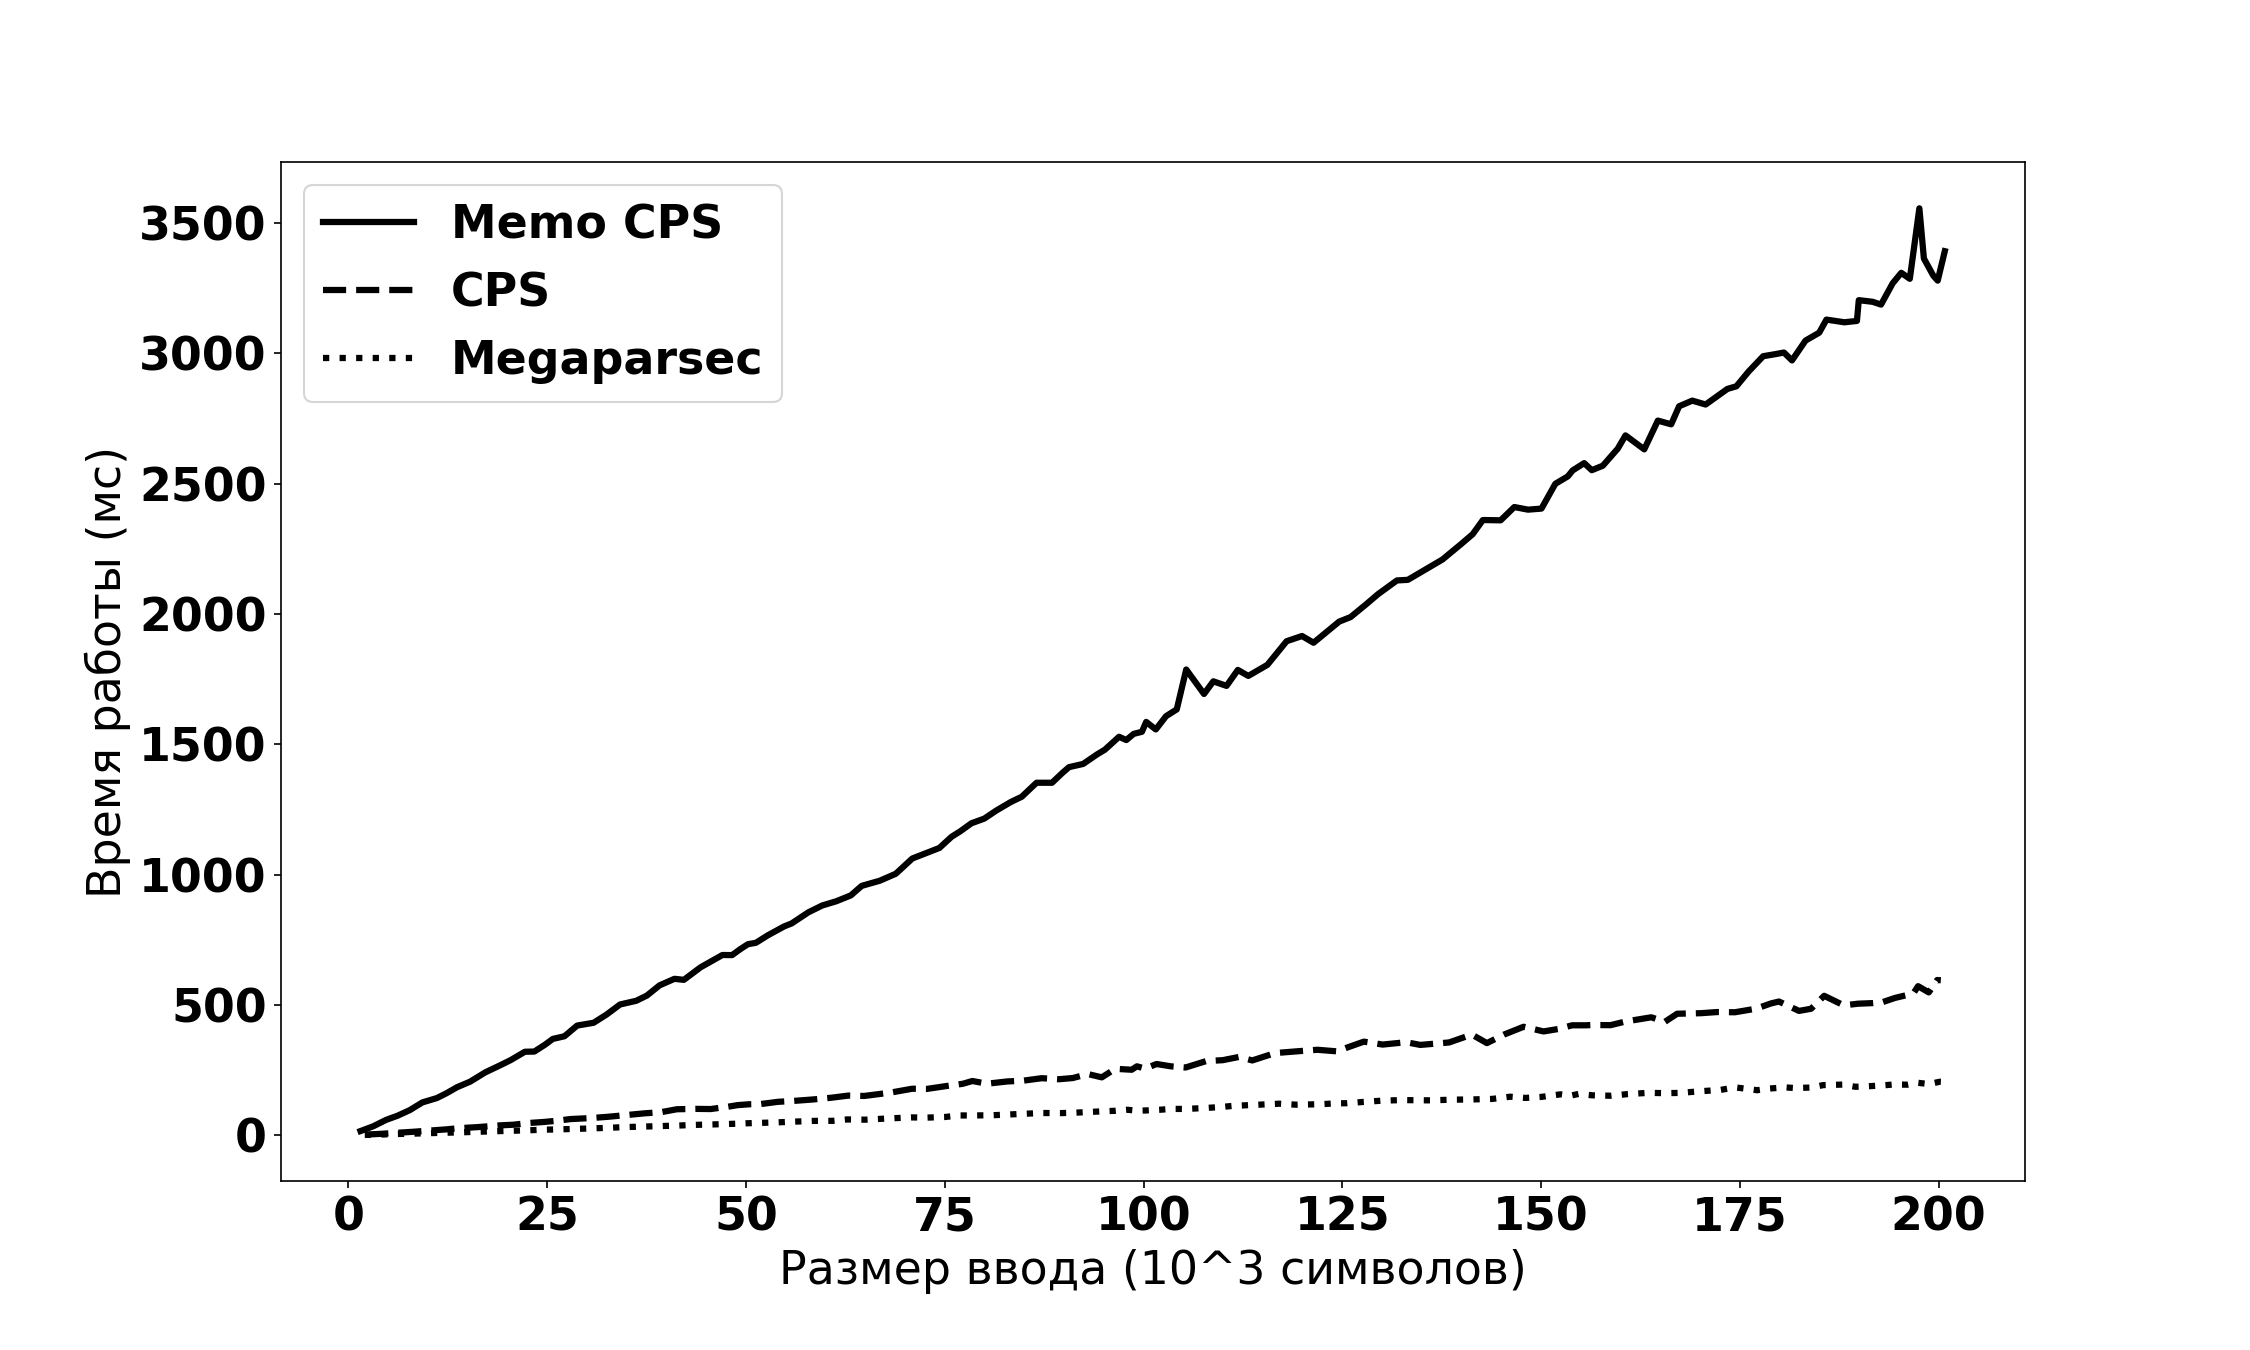
\includegraphics[width=0.8\paperwidth]{./images/megaparsec_comparison.png}
\end{figure}

Существенным недостатком мемоизированных CPS-парсеров является увеличенное потребление памяти, которое связано с
необходимостью хранить промежуточные значения разбора. На таблице \ref{tab:arith_memory} приведено потребление памяти
тремя парсерами при разборе арифметических выражений длиной 2000, 50000, 100000 и 200000 символов. По данным из таблицы
видно, что потребление памяти мемоизированным CPS-парсером растёт линейно в зависимости от длины ввода.

\begin{table}[!h]
  \caption{Потребление памяти в зависимости от длины разбираемого арифметического выражения}\label{tab:arith_memory}
  \centering
  \begin{tabular}{|*{4}{c|}}\hline
    --     & Memo CPS & Megaparsec & CPS   \\\hline
    2000   & 12 МБ    & 6 МБ       & 7 МБ  \\\hline
    50000  & 137 МБ   & 14 МБ      & 28 МБ \\\hline
    100000 & 271 МБ   & 19 МБ      & 43 МБ \\\hline
    200000 & 578 МБ   & 29 МБ      & 71 МБ \\\hline
  \end{tabular}
\end{table}

\section{Разбор контекстно-свободных грамматик}\label{sec:context_free}

\begin{figure}[!h]
  \caption{Не $LL(k)$ грамматика}\label{fig:not_llk_grmmar}
  \[
      \begin{array}{lll}
          A & \to & a A x \\
            &     & a A y \\
            &     & \epsilon
      \end{array}
  \]
\end{figure}

Как показано в разделе \ref{sec:arith_expr}, для арифметических выражений, чья грамматика записана в нелеворекурсивном
виде, можно не использовать мемоизацию, при этом асимптотика времени работы парсера не изменится. Однако это суждение верно не
для любой грамматики. Как было замечено в разделе \ref{sec:cps_algorithm} алгоритм CPS-парсеров гарантирует полиномиальное время
работы парсера. Приведём пример, когда мемоизация даёт выигрыш даже для нелеворекурсиных парсеров. Рассмоторим
грамматику с рисунка \ref{fig:not_llk_grmmar}. Очевидно, что она не $LL(k)$: какое бы число символов
\lstinline{'a'} парсер не принимал во внимание, существует строка, на которой он не сможет  определить, какое
правило вывода для нетерминала $A$ применить. Время работы обычного комбинаторного парсера с
возвратом при разборе такой грамматики равно $O(2^n)$ на вводах типа $a^n(x|y)^n$. Это время
работы свойственно в том числе и Megaparsec, и разработанному парсеру при отсутствии мемоизации. Время работы разработанного 
немемоизированного CPS-парсера показано на графике <<Unmemoized parser>> с рисунка \ref{fig:notllk_plot}. Тем не менее
при  использовании мемоизированных CPS-парсеров время разбора становится квадратичным, что можно видеть на графике
<<Memoized parser>> c рисунка \ref{fig:notllk_plot}. Графики <<fit>> --- это графики функций, апроксимированных  на
основании полученных измерений.

\begin{figure}[!h]
  \caption{Скорость работы CPS-парсера на не $LL(k)$ грамматике}\label{fig:notllk_plot} %% Показать график с экспонентой для немемоизированной парсера
  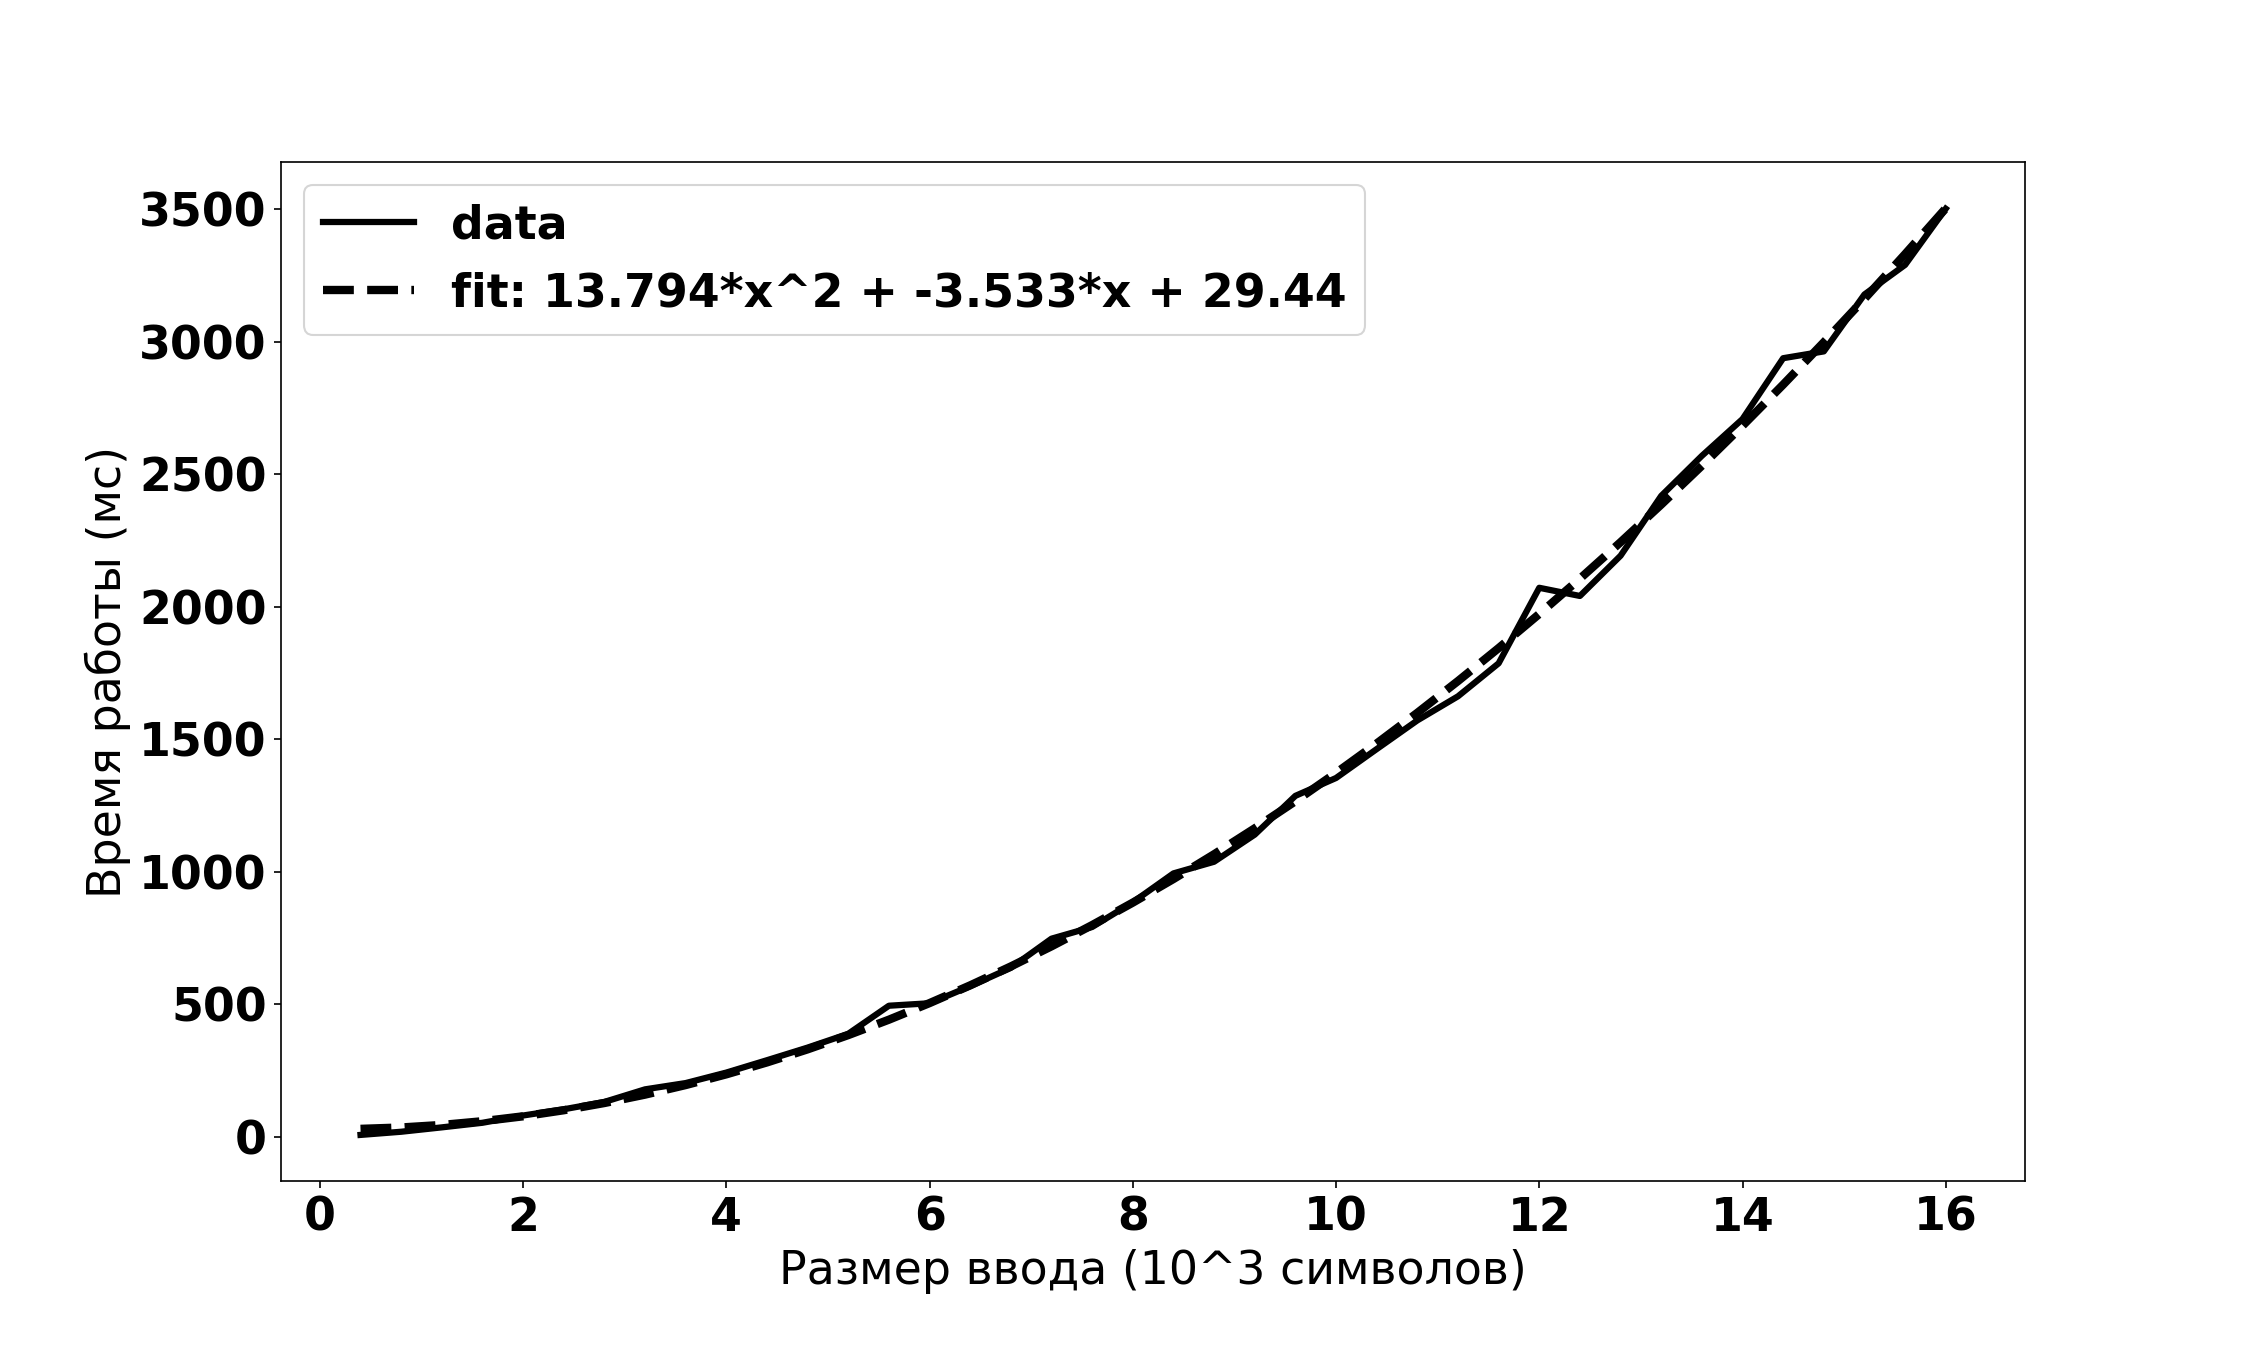
\includegraphics[width=0.8\paperwidth]{./images/notllk_memo.png}
  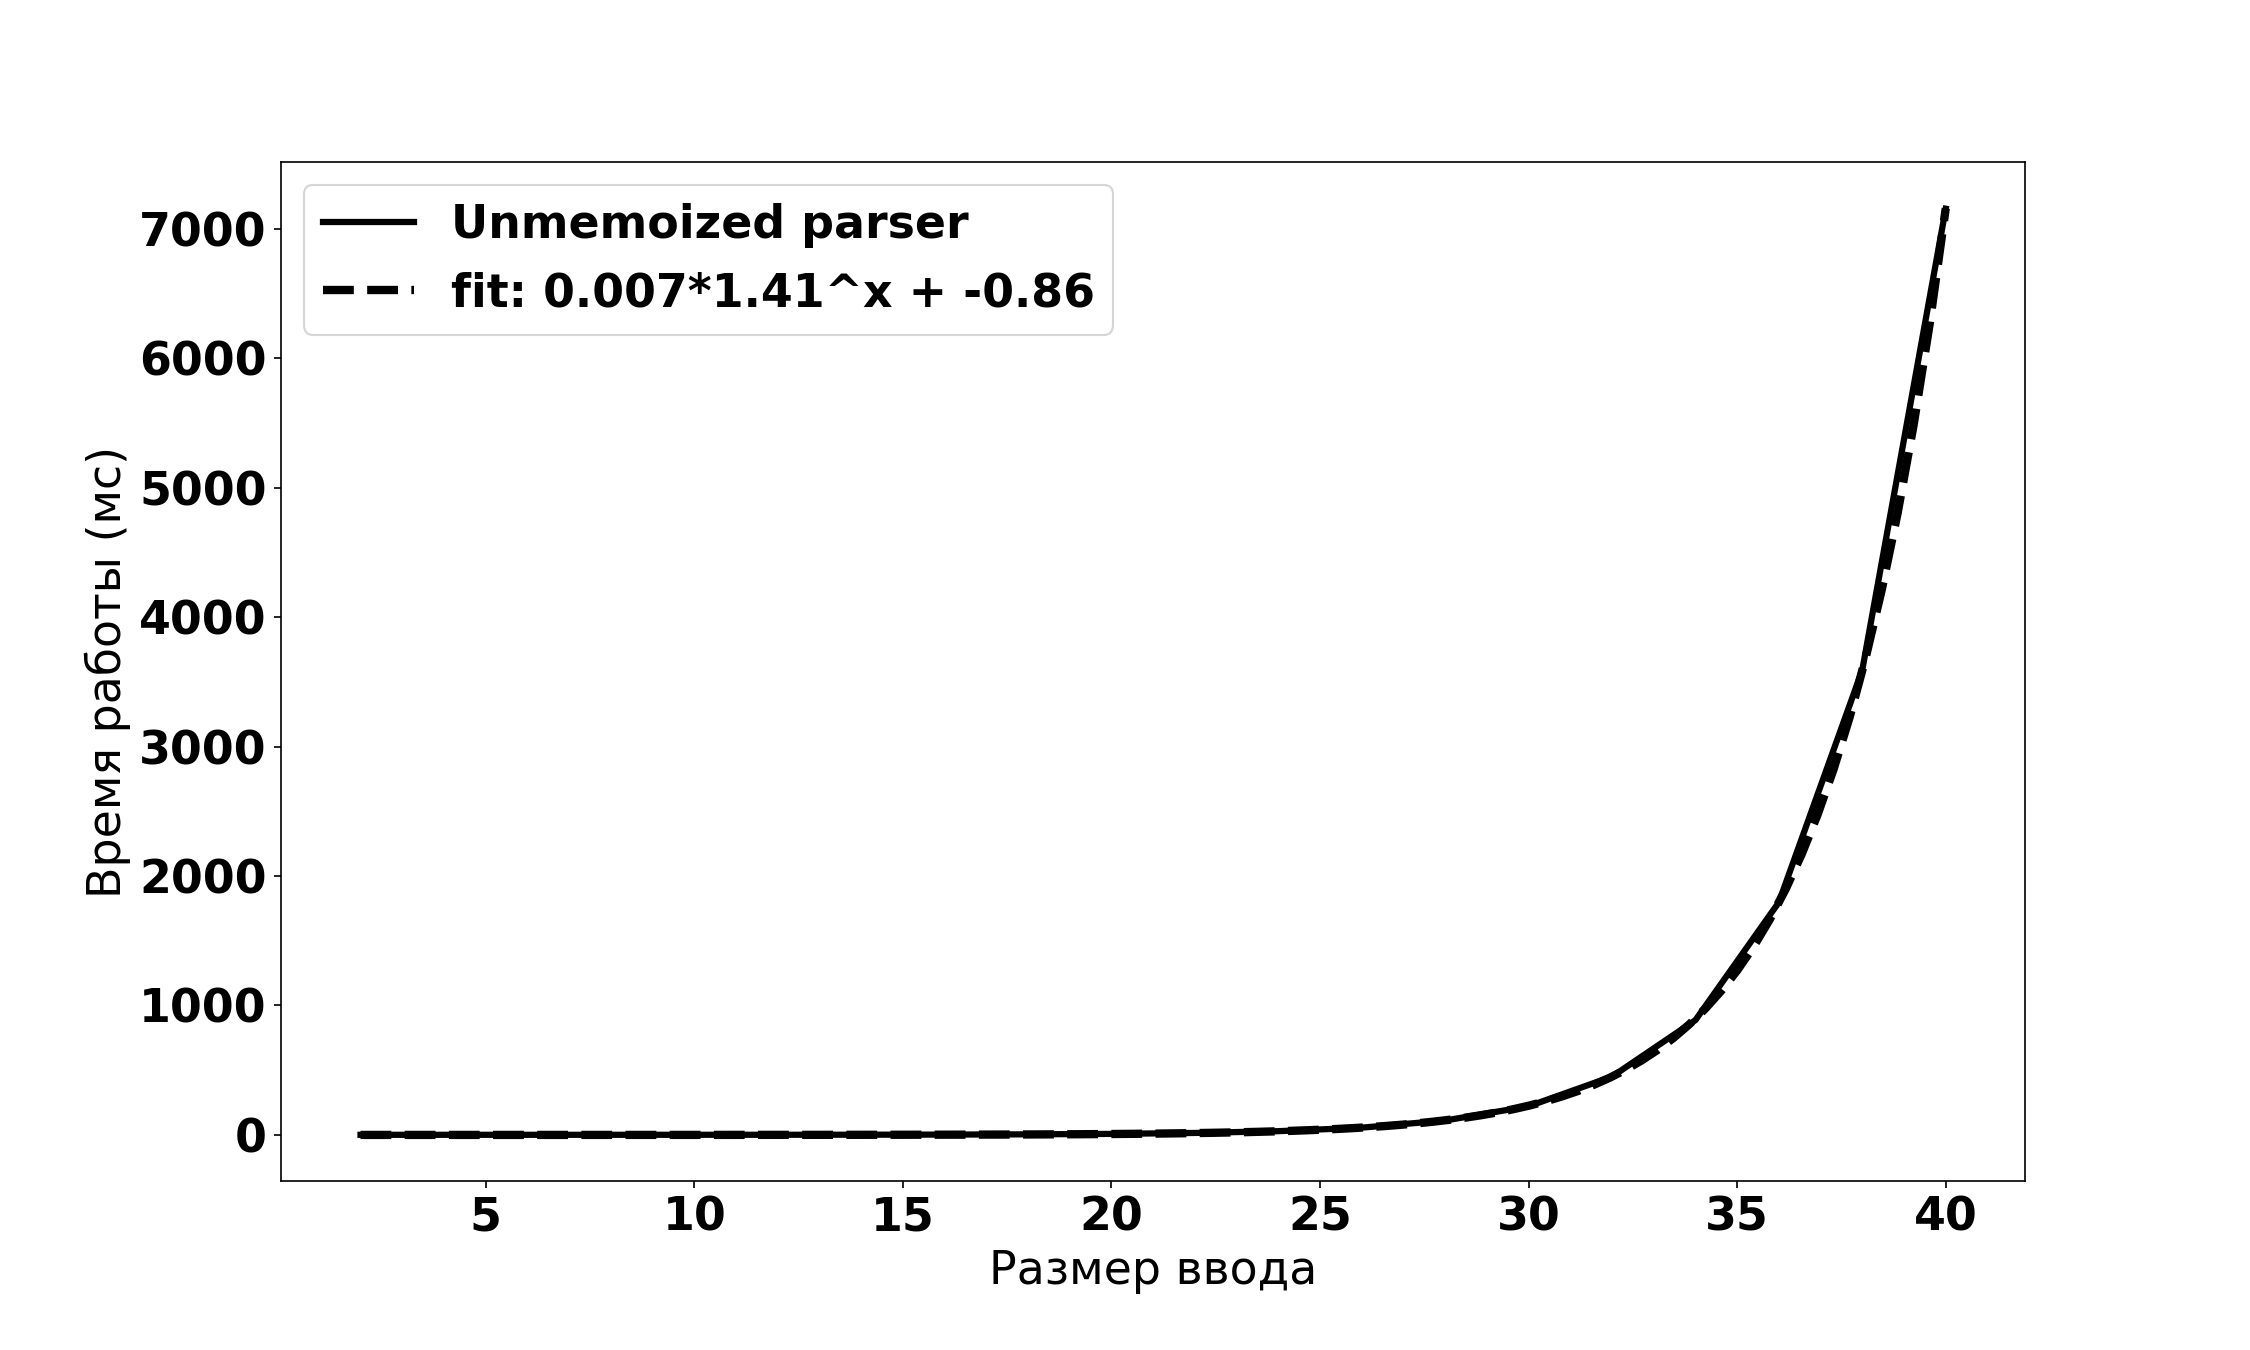
\includegraphics[width=0.8\paperwidth]{./images/notllk_unmemo.png}
\end{figure}

\section{Разбор не контекстно-свободных грамматик}\label{sec:non_context_free}

Важной особенностью написанного парсера является его монадичность, которая позволяет описывать с его помощью не только 
КСГ. Известно, что язык, порождаемый множеством строк, задаваемых регулярных выражением $a^kb^kc^k$ для любого натурального $k$, 
не является контекстно-свободным. Тем не менее с помощью разработнной библиотеки такой язык можно разобрать, используя парсер с листинга 
\ref{lst:anbncn_parser}.

\begin{lstlisting}[language=Haskell,float=!h,caption={Парсер $a^kb^kc^k$},label={lst:anbncn_parser}]
  anbncn :: Parser (ParserState String) String
  anbncn = do
    a <- some (single 'a')
    b <- replicateM (length a) (single 'b')
    c <- replicateM (length a) (single 'c')
    eof
    return $ a ++ b ++ c
\end{lstlisting}

\section{Сравнение свойств разработанной библиотеки с существующими интсрументами}\label{sec:comparison_table}

В таблице \ref{tab:comparison} представлено сравнительнение свойств некоторых инструментов синтаксического анализа,
которые существуют на данный момент. Выбранные для сравнения иструменты либо популярны, либо обладают уникальными
свойствами. Важно заметить, что ни один из существующих комбинаторных парсеров не поддерживает левую рекурсию,
пользовательскую семантику и при этом способен разбирать любую контекстно-свободную грамматику. Библиотека, написанная в 
рамках ВКР, называется в таблице <<\textit{CPS}>>.

Проблема таких инструментов как ANTLR и Bison заключается в том, что они являются генераторами, а не комбинаторами парсеров.
Это приводит к проблемам, описанным в разделе \ref{sec:parser_combinators_advantages}. 

Проблема Parsley~\cite{willis_staged_2020} и подобных инструментов заключается во-первых в меньшей выразительной мощи в
сравнении с монадическими инструментами анализа, а во вторых в отcутствии поддержки левой рекурсии.
Интруметы типа PyParsing используют алгоритм Packrat~\cite{ford_parsing_2004}, который подходит для разбора PEG, что
делает невозможным в общем случае комбинировать парсеры, написанные с использование Packrat.
Существующие монадические комбинаторные парсеры типа MegaParsec используют поиск с возвратом только в случае, когда это явно
указано пользователем. Вместе с тем возврат без мемоизаиции приводит к экспоненциальному времени разбора на некоторых КСГ, 
что было показано в разделе \ref{sec:current_parser_combinators_problems}.

Важно рассмотреть библиотеку Meerkat~\cite{johnson_memoization_1995}. В её основе лежит тот же алгоритм, который используется для
библиотеки, написанной	в рамках ВКР. Тем не менее Meerkat оптимизирован для разбора неоднозначных грамматик, в связи с
этим результатом разбора с использованием Meerkat служит SPPF (shared packed parse forest), что не позволяет пользователю
задавать свою семантику для разбора.

\begin{table}[H]
  \caption{Сравнительный анализ некоторых инструментов синтаксического анализа}\label{tab:comparison}
  \centering
  \setlength{\tabcolsep}{0.38em}
  \small
  \begin{tabular}{|c|cc|ccccc|}
    \hline
                                                                          & \multicolumn{1}{c|}{ANTLR} & Bison & \multicolumn{1}{c|}{Parsley}   & \multicolumn{1}{c|}{PyParsing} & \multicolumn{1}{c|}{MegaParsec}   & \multicolumn{1}{c|}{Meerkat} & \textit{CPS} \\ \hline
    Тип                                                                   & \multicolumn{2}{c|}{генератор}     & \multicolumn{5}{c|}{комбинатор}                                                                                                                                           \\ \hline
    Вид                                                                   & \multicolumn{2}{c|}{}              & \multicolumn{1}{c|}{апликатив} & \multicolumn{4}{c|}{монада}                                                                                                              \\ \hline
    Класс грамматик                                                       & \multicolumn{1}{c|}{LL(*)} & КСГ   & \multicolumn{1}{c|}{КСГ}       & \multicolumn{1}{c|}{PEG}       & \multicolumn{3}{c|}{КСГ}                                                                                \\ \hline
    Время работы                                                          & \multicolumn{1}{c|}{O(n)}  & O(n³) & \multicolumn{1}{c|}{O(n³)}     & \multicolumn{1}{c|}{O(n)}      & \multicolumn{1}{c|}{O(n) -- O(eⁿ)} & \multicolumn{1}{c|}{O(n³)}   & O(n³)        \\ \hline
    Лев. рекурсия                                                         & \multicolumn{1}{c|}{Нет}   & Да    & \multicolumn{1}{c|}{Нет}       & \multicolumn{1}{c|}{Нет}       & \multicolumn{1}{c|}{Нет}          & \multicolumn{1}{c|}{Да}      & Да           \\ \hline
    \begin{tabular}[c]{@{}c@{}}Пользовательская\\  семантика\end{tabular} & \multicolumn{1}{c|}{Да}    & Да    & \multicolumn{1}{c|}{Да}        & \multicolumn{1}{c|}{Да}        & \multicolumn{1}{c|}{Да}           & \multicolumn{1}{c|}{Нет}     & Да           \\ \hline
  \end{tabular}
\end{table}

\startconclusionpage

В рамках работы были рассмотрены недостатки существующих подходов к синтаксическому анализу формальных языков,
заключающиеся в невозможности произвольной композиции парсеров. Было выявлено, что наиболее удачной формой для описания
парсеров, поддерживающих композицию, являются комбинаторные парсеры. Тем не менее было показано, что существующие
комбинаторные парсеры не обладают в полной мере свойством композиционности в силу их чувствительности к левой рекурсии,
а также неспособностью большинства из них разбирать любые КСГ за полиномиальное время. В рамках работы на основе
рекогнайзеров Джонсона	был разработан комбинаторный парсер, поддерживающий левую рекурсию и разбирающий любые
однозначные КСГ за полиномиальное время. Экспериментально было проверено, что разработанный парсер удовлетворяет всем
необходимым свойствам. Таким образом, были  выполнены все задачи ВКР. Разработанная в рамках ВКР библиотека обладает
всеми заявленными свойствами.

Полученный результат можно применять для переиспользования частей парсеров, написанных для разбора различных языков,
кроме того он открывает подход к модульному написанию парсеров, при котором парсеры более сложных языков можно собирать
из парсеров для простых языков. Например, с помощью разработанной библиотеки предположительно возможно закодировать
парсеры для семейства вложенных друг в друга языков с высокой степенью переиспользования кода. В дальнейшем планируется, 
используя написанную библиотеку, разработать парсер нетривиального языка программирования путём добавления к ядру языка 
дополнительных модулей. Кроме того в планах добавить обработку ошибок разбора.

\printmainbibliography

\end{document}
